% DO NOT COMPILE THIS FILE DIRECTLY!
% This is included by the other .tex files.

\begin{frame}[t,plain]
\titlepage
\end{frame}

\begin{frame}[t]{Resource Allocation}
    \begin{itemize}
        \item<2-> Allocation of scarce resources to \textbf{customers} under some constraints
        \item<3-> Application:
        \item<4->[ ]
        \begin{figure}
            \begin{subfigure}[b]{0.45\textwidth}  
                \centering
                
\includegraphics[width=2cm]{auction.eps}
                \caption*{Auctions}
                \label{fig:my_label}
            \end{subfigure}
            \begin{subfigure}[b]{0.45\textwidth}    
                \centering
                
\includegraphics[width=2cm]{pie-chart.eps}
                \caption*{Cake Cutting}
                \label{fig:my_label}
            \end{subfigure}
            \begin{subfigure}[b]{0.45\textwidth}     
                \centering
                
\includegraphics[width=2cm]{cpu.eps}
                \caption*{Job Scheduling}
                \label{fig:my_label}
            \end{subfigure}
            \begin{subfigure}[b]{0.45\textwidth}      
                \centering
                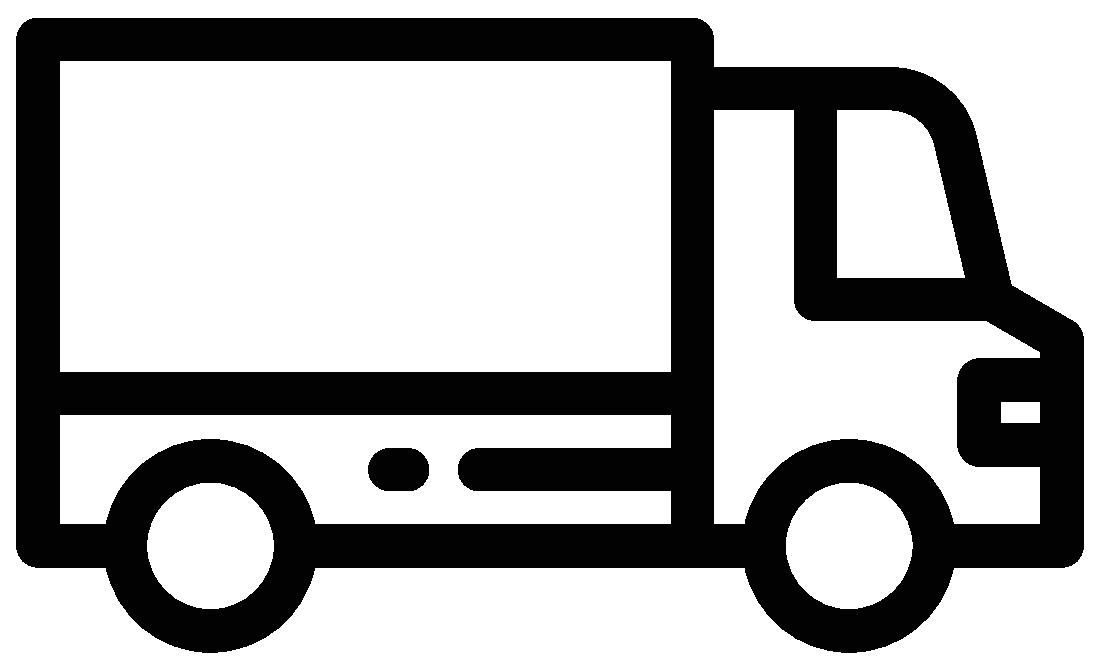
\includegraphics[width=2cm]{delivery-truck.eps}
                \caption*{Delivery}
                \label{fig:my_label}
            \end{subfigure}
        \end{figure}
    \end{itemize}    
\end{frame}

\begin{frame}[t]{Resource Allocation Types}
    \begin{itemize}
        \item<2-> Divisible Resource Allocation
            \begin{itemize}
                \item<3-> Example: cake cutting problem
            	\item<4-> The question: \emph{fair division} of divisible resources
            	\item<5-> Mostly studied in  economics, game theory, and sociology
            \end{itemize}
        \item<6-> Indivisible Resource Allocation (\alert{IRA})
            \begin{itemize}
                \item<7-> Example: Auctions, Scheduling, Vehicle Routing
                \item<8-> Combinatorial nature of the allocation
                \item<9-> Mostly studied in operation research, combinatorial optimization, and computer science
            \end{itemize}  
    \end{itemize}
\end{frame}

\begin{frame}{In This Presentation}
  \tableofcontents
\end{frame}

%__________________________________________________________________________________
\section{Skill Vehicle Routing Problem}
\frame{\textbf{\insertsection}}

\begin{frame}[t]{Introduction (1)}
    \begin{minipage}[t]{0.48\textwidth}
        \begin{itemize}
            \item<1-> Set of \textbf{customers} $S$
            \item<2-> Skill requirement $q_j$,  $\forall j \in S$
            \item<3-> Fleet of vehicles (\textbf{drivers}) $D$
            \item<4-> Set of skills $K_i$ $\forall i \in D$
            \item<5-> Special node \emph{depot}, $r \in S$
            \item<6-> Metric graph $G = (S, \, E)$
            \item<7-> Cost function $c:E \rightarrow \bR^+$ for every pair of nodes
        \end{itemize}
    \end{minipage}
    \begin{minipage}[t]{0.48\textwidth}
        \begin{figure}
            \centering
            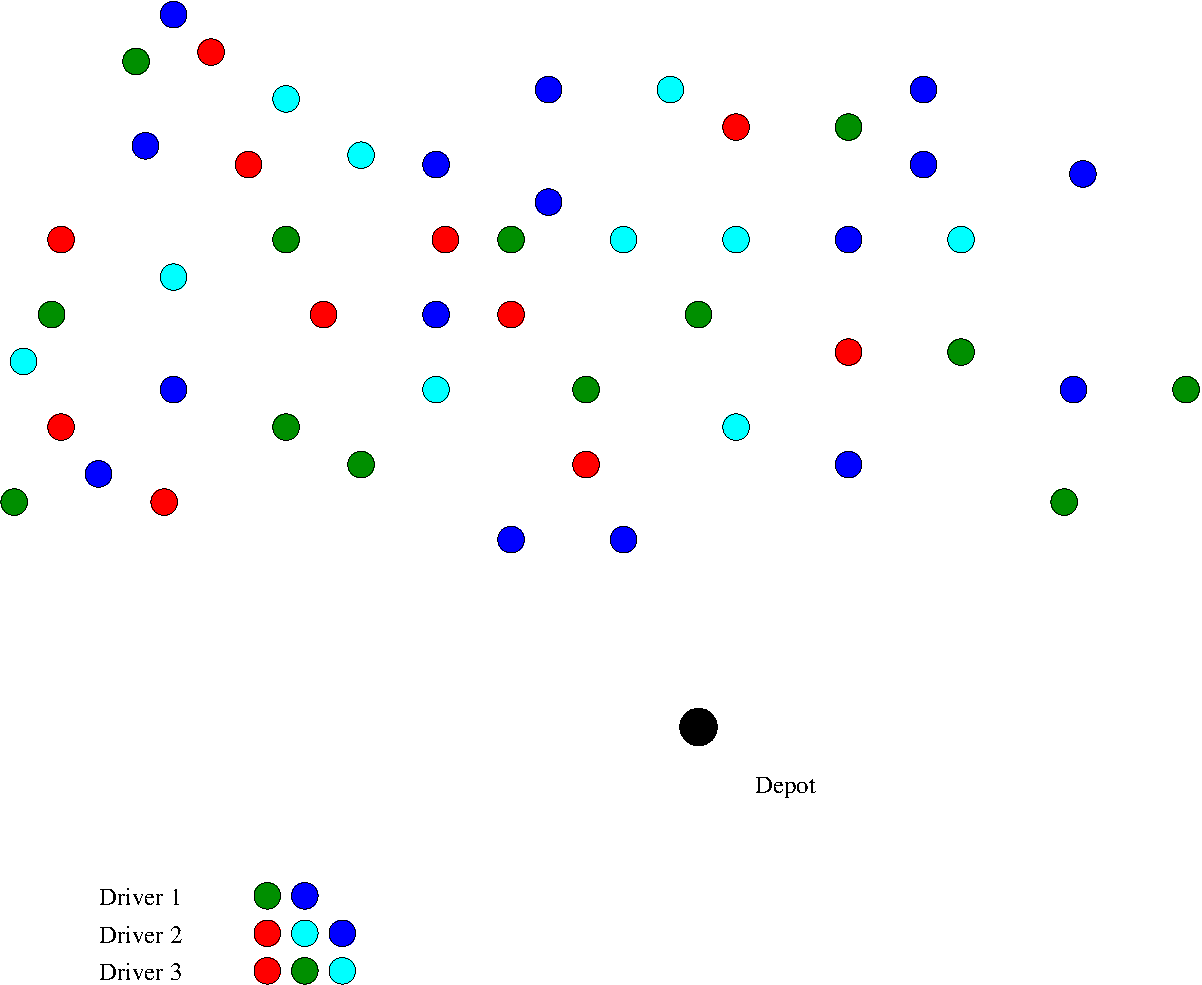
\includegraphics[width=5cm]{VRPSS01.pdf}
            \caption{SVRP}
            \label{fig:VRPSS01}
        \end{figure}            
    \end{minipage}
\end{frame}

\begin{frame}[t]{Introduction (1)}
    \begin{minipage}[t]{0.48\textwidth}
        \begin{itemize}
            \item Set of \textbf{customers} $S$
            \item Skill requirement $q_j$,  $\forall j \in S$
            \item Fleet of vehicles (\textbf{drivers}) $D$
            \item Set of skills $K_i$ $\forall i \in D$
            \item Metric graph $G = (S, \, E)$
            \item Special node \emph{depot}, $r \in S$
            \item Cost function $c:E \rightarrow \bR^+$ for every pair of nodes
        \end{itemize}
    \end{minipage}
    \begin{minipage}[t]{0.48\textwidth}
        \begin{figure}
            \centering
            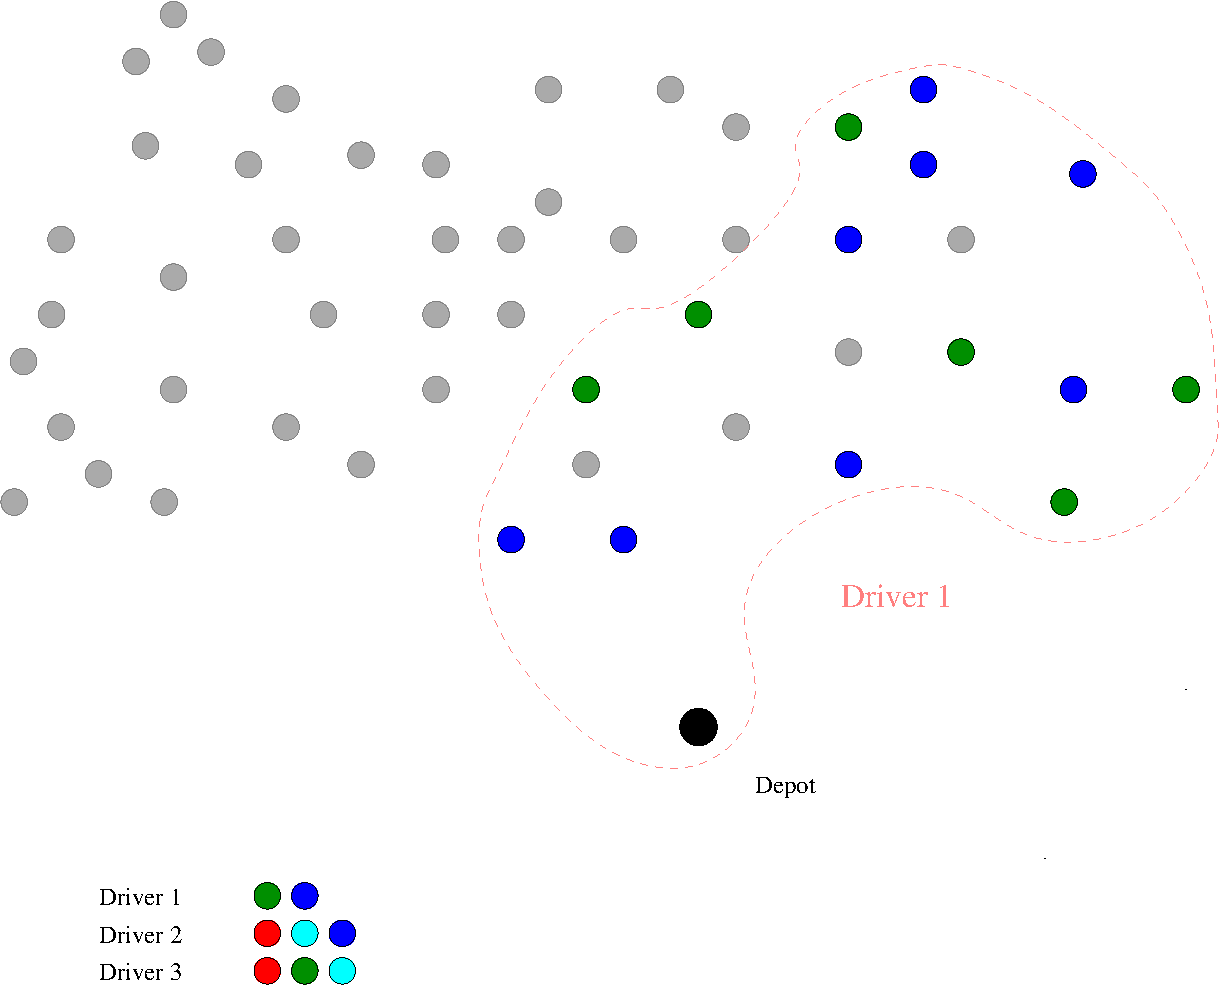
\includegraphics[width=5cm]{VRPSS02.pdf}
            \caption{SVRP}
            \label{fig:VRPSS02}
        \end{figure}            
    \end{minipage}    
\end{frame}

\begin{frame}[t]{Introduction (1)}
    \begin{minipage}[t]{0.48\textwidth}
        \begin{itemize}
            \item Set of \textbf{customers} $S$
            \item Skill requirement $q_j$,  $\forall j \in S$
            \item Fleet of vehicles (\textbf{drivers}) $D$
            \item Set of skills $K_i$ $\forall i \in D$
            \item Metric graph $G = (S, \, E)$
            \item Special node \emph{depot}, $r \in S$
            \item Cost function $c:E \rightarrow \bR^+$ for every pair of nodes
        \end{itemize}
    \end{minipage}
    \begin{minipage}[t]{0.48\textwidth}
        \begin{figure}
            \centering
            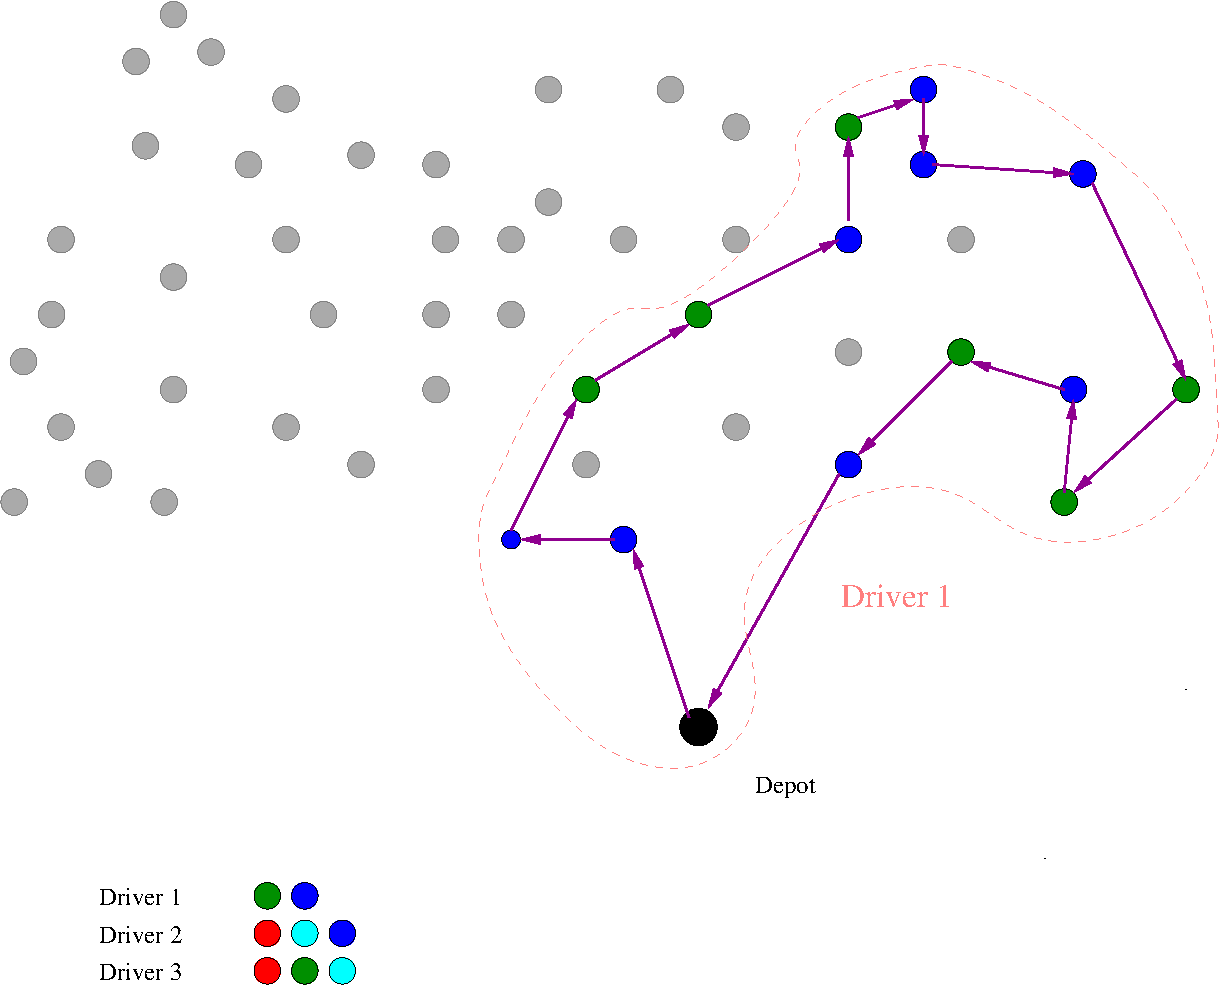
\includegraphics[width=5cm]{VRPSS03.pdf}
            \caption{SVRP}
            \label{fig:VRPSS02}
        \end{figure}            
    \end{minipage}    
\end{frame}

\begin{frame}{Introduction (2)}
\begin{itemize}
    \item<1-> Goal: to find \textbf{tours} (routes that start and end at $r$) and assign them to drivers such that:
    \begin{itemize}
        \item<2-> The union of all the tours cover $S$
        \item<3-> The drivers can served the customers assigned to them
        \item<4-> The total travel distance is minimized
    \end{itemize}
    \item<5-> SVRP has immediate applications in logistics and transportation
        \begin{itemize}
            \item<6-> Transport costs account for 10\% of the total cost of a product
            \item<7-> Manual optimization of the transport cost becomes infeasible as the scale grows
        \end{itemize}
    \item<7-> We seek to solve SVRP \textbf{computationally}
\end{itemize}
\end{frame}


\begin{frame}[t]{Solution Methods}
    \begin{itemize}
        \item<1-> Metaheuristics:
            \begin{itemize}
                \item<2-> Tabu search
                \item<3-> Simulated annealing
                \item<4-> \ldots
            \end{itemize}
        \item<5-> Linear Programming:
            \begin{itemize}
                \item<6-> Goal: obtain minimum-cost solutions or lower and upper bounds
                \item<7-> an LP-relaxation used in a branch-and-bound algorithm
                \item<8-> Integrality gap plays an important role
                \item<9-> Question: a formulation with small gap?
                \item<10-> Answer: \textbf{Configuration LP}
            \end{itemize}
    \end{itemize}
\end{frame}

\begin{frame}[t]{Configuration LP (1)}
    \begin{itemize}
        \item<1-> First used in the context of Bin Packing problems
        \item<2-> For every driver $i \in D$, $\cT(i)$ is the set of tours $i$ can serve        
        \item<3-> For every driver $i \in D$ and every tour $T \in \cT(i)$:
        \[
            z_{i, T} =
                \begin{cases}
                    1 & \text{if driver $i$ visits the vertices in the tour $T$} \\
                    0 & \text{otherwise}
                \end{cases}
        \]
    \end{itemize}
\end{frame}
\begin{frame}[t]{Configuration LP (2)}
    \label{CLP2}
    \begin{itemize}
        \item<1->[ ] \begin{align}
            \text {min } \label{cg_obj}	 \sum_{ i, 	T \in \cT(i) } z_{i, T} & \cdot C(T) &    &  \\
            \text{subject to }             & & \nonumber  \\
            \label{const:cg1}       \sum_{ T \in \cT(i) } z_{ i, T } & = 1  &   \forall i \in D \\
            \label{const:cg2}       \sum_{ i, T \in \cT(i): T \ni j } z_{ i, T } & \geq 1   &   \forall j \in S \\
            \label{consT:cg3}       z_{ i, T } & \in \{0,\, 1\}    & \forall \, i \in D, \, \forall \, T \in \cT(i) 
        \end{align}        
        \hyperlink{our_method_bp}{\beamergotobutton{Branch-and-Price}}
    \end{itemize}
\end{frame}

\begin{frame}[t]{Configuration LP (3)}
    \begin{itemize}
        \item<1-> Advantage:
            \begin{itemize}
                \item<2-> Small integrality gap
            \end{itemize}
        \item<3-> Disadvantage: 
            \begin{itemize}
                \item<4-> Exponential number of variables
            \end{itemize}
        \item<5-> Common technique for dealing with LP formulations with a large number of constraints: \textbf{Delayed Column Generation}
            \begin{itemize}
                \item<6-> Do not introduce all the variables at once
                \item<7-> Solve LP relaxation on a subset of variables (columns)
                \item<8-> Detect and introduce columns that can improve the solution: \textbf{reduced-cost columns}
                \item<9-> Used extensively for Vehicle Routing Problems with Time Windows
            \end{itemize}
    \end{itemize}
\end{frame}

\begin{frame}[t]{Our Contributions}
    \label{our_method_bp}
    \begin{itemize}
        \item<1-> A \alert{Branch-and-Price} algorithm: 
        \item<2-> Use column generation in a branch-and-bound framework
        \item<3-> Detect the reduced-cost columns (\textbf{Pricing} subproblem)
            \begin{itemize}
                \item<4-> Heuristic: a \alert{local search} algorithm 
                \item<5-> Exact solutions: \alert{Prize-Collecting TSP}
            \end{itemize}
        \item<6-> Use both the heuristic and exact solutions to improve upper and lower bounds \hyperlink{CLP2}{\beamergotobutton{Config. LP}}        
        \item<7-> Future projects:
            \begin{itemize}
                \item<8-> Benchmarking heuristics and metaheuristics
                \item<9-> Improving the branch-and-price with heuristics
            \end{itemize}
    \end{itemize}
\end{frame}

%__________________________________________________________________________________
\section{Prize Collecting TSP}
\frame{\textbf{\insertsection}}

\begin{frame}[t]{Introduction}

\begin{itemize}
\item<1-> A variant of the Traveling Salesman Problem (TSP)
\item<2-> Metric graph $G = (S, \, E)$ (on a Euclidean plane) 
\item<3-> A special node depot, $r \in S$
\item<4-> A cost function $c:E \rightarrow \bR^+$ for every pair of nodes
\item<5-> A \textbf{prize} function $\beta:S \rightarrow \bR^+$ for every node
\item<6-> Objective: Find a tour covering the depot and a \emph{subset} of nodes, maximizing the sum of prizes minus the sum of costs

\end{itemize}
\end{frame}

\begin{frame}[t]{Introduction (2)}

\begin{itemize}
\item An instance of the Prize Collecting TSP:
\begin{figure}
	\centering
	\begin{tikzpicture}
        
        \draw (0, 0) node[circle, inner sep=1pt, fill=black, label={below:{$depot$}}] (D) {}; 
        \draw (1, 1) node[circle, inner sep=1pt, fill=black] (A) {}; 
        \draw (3, 2) node[circle, inner sep=1pt, fill=black] (B) {}; 
        \draw (-3, 3) node[circle, inner sep=1pt, fill=black] (C) {}; 
        \draw (-1, 4) node[circle, inner sep=1pt, fill=black] (E) {}; 
        \draw (0, 3) node[circle, inner sep=1pt, fill=black] (F) {}; 
        \draw (2, 3) node[circle, inner sep=1pt, fill=black] (G) {}; 
         \draw (-3, 1) node[circle, inner sep=1pt, fill=black, label={below:{$v$}}] (v) {}; 
        \draw (-2, 2) node[circle, inner sep=1pt, fill=black, label={below:{$u$}}] (u) {};         
        \node at (-2.5, 1.5) (m) {};
        \node at (-4, 1.5) (n) {$c_{uv}$};
        
        \draw [->, color = red] (m) to [bend right = 45] (n);
        \draw [fill = blue, dashed, thick] (u) to (v);

    	\node[above = 0.2cm] at (-2, 2) {$\beta_u$};
	\end{tikzpicture}
    \caption{Prize Collecting TSP}
    \label{fig:intersect_intervals}
\end{figure}
\end{itemize}
\end{frame}

\begin{frame}[t]{Introduction (3)}

\begin{itemize}
\item Solution value $ = (6 + 2 + 7 + 10 + 4) - (3.2  + 1.4 + 2.2 + 3.2 + 2.2 + 1.4) = $ \alert{15.4}
\begin{figure}
	\centering
	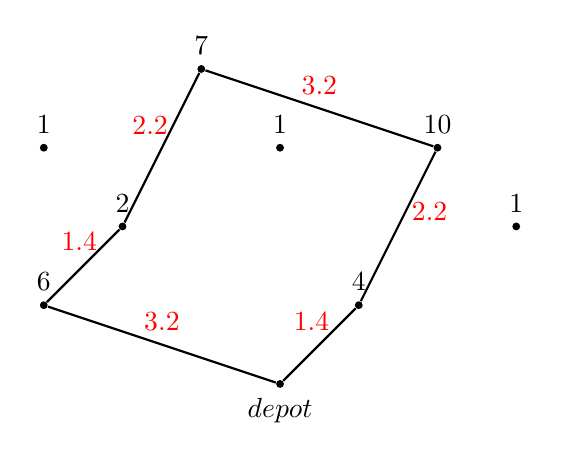
\begin{tikzpicture}
        
        \draw (0, 0) node[circle, inner sep=1pt, fill=black, label={below:{$depot$}}] (D) {}; 
        \draw (1, 1) node[circle, inner sep=1pt, fill=black, label = {above:{4}}] (A) {}; 
        \draw (3, 2) node[circle, inner sep=1pt, fill=black, label = {above:{1}}] (B) {}; 
        \draw (-3, 3) node[circle, inner sep=1pt, fill=black, label = {above:{1}}] (C) {}; 
        \draw (-1, 4) node[circle, inner sep=1pt, fill=black, label = {above:{7}}] (E) {}; 
        \draw (0, 3) node[circle, inner sep=1pt, fill=black, label = {above:{1}}] (F) {}; 
        \draw (2, 3) node[circle, inner sep=1pt, fill=black, label = {above:{10}}] (G) {}; 
         \draw (-3, 1) node[circle, inner sep=1pt, fill=black, label = {above:{$6$}}] (v) {}; 
        \draw (-2, 2) node[circle, inner sep=1pt, fill=black, label = {above:{$2$}}] (u) {};                 
        \draw [fill = blue, thick] (D) to (v) to (u) to (E) to (G) to (A) to (D);
        \node [above = 0.05cm, color = red] at (-1.5, 0.5) {3.2};
        \node [above = 0.07cm, color = red] at (-2.55, 1.5) {1.4};
        \node [above = 0.05cm, color = red] at (-1.65, 3) {2.2};
        \node [above = 0.05cm, color = red] at (0.5, 3.5) {3.2};
        \node [above = 0.05cm, color = red] at (1.9, 1.9) {2.2};
        \node [above = 0.05cm, color = red] at (0.4, 0.5) {1.4};
        
	\end{tikzpicture}
    \caption{A feasible solution to PCTSP}
    \label{fig:intersect_intervals}
\end{figure}
\end{itemize}
\end{frame}

\begin{frame}[t]{Solution Methods}
    \begin{itemize}
        \item<1-> PCTSP may arise as subproblem in a column generation technique for many vehicle routing problems
        \item<2-> SVRP is one example
        \item<3-> We seek:
            \begin{itemize}
                \item<4-> Fast heuristics that provide near-optimal solutions
                    \begin{itemize}
                        \item<5-> These solutions can be used as reduced-cost columns for SVRP
                        \item<6-> Normally based on local search
                    \end{itemize}
                \item<7-> Exact solutions that provide bounds for SVRP
                    \begin{itemize}
                        \item<8-> Based on LP formulations with small integrality gap
                        \item<9-> Used in a branch-and-bound framework
                    \end{itemize}
                    
            \end{itemize}
    \end{itemize}
\end{frame}


\begin{frame}[t]{Related Work}
\begin{itemize}
    \item<1-> Metaheuristics:
        \begin{itemize}
            \item<2-> A local search algorithm is due to Chaves and Lorena
        \end{itemize}
        \item<3-> Linear Programming:
        \begin{itemize}
            \item<4-> Some formulations with exponential number of constraints exhibit low integrality gaps for TSP-like problems
            \item<5-> Normally a mix of cutting plane method and branch-and-bound is used: \textbf{Branch-and-Cut}
            \item<6-> Gendreau et al., Fischetti et al., and B\'{e}rub\'{e} et al. provide Branch-and-Cut algorithms for variants of the problem
        \end{itemize}
\end{itemize}
\end{frame}

\begin{frame}[t]{ILP Formulation (1)}
    \begin{itemize}
        \item<1-> Two sets of decision variables:
        \item<2-> For every vertex $i \in S$:
        \[
            y_j =
                \begin{cases}
                    1 & \text{if vertex $j$ is selected in the optimal tour} \\
                    0 & \text{otherwise}
                \end{cases}
        \]       
        \item<3-> For every edge $e \in E$:
        \[
            x_e =
                \begin{cases}
                    1 & \text{if edge $e$ is selected in the optimal tour} \\
                    0 & \text{otherwise}
                \end{cases}
        \]        
    \end{itemize}
\end{frame}

\begin{frame}[t]{ILP Formulation (2)}
    \begin{align} 
        \text {max } \label{pctsp_obj}     & \sum_{j\in S} \beta_j y_j  -     \sum_{e\in E} c_e x_e &
        \\
        \text{subject to } \nonumber    &  & \\
        \label{const:pctsp1}               & \sum_{e \in \delta(i)} x_e = 2 y_{i}  & \forall i \in S \\
        \label{const:pctsp2}               & \sum_{e \in E(V) } x_e \leq \sum_{i \in V \backslash\{ k \}} y_{i} & \forall k \in V, V\subseteq S' \\
        \label{const:pctsp3}               & y_r = 1 \\
        \label{const:pctsp4}               & x_e \in \{0, \, 1\}, \, y_j \in \{0, \, 1\}  
    \end{align}
\end{frame}

\begin{frame}[t]{ILP Formulation (3)}
    \begin{itemize}
        \item<1->[ ]
        \[  \sum_{e \in E(V) } x_e \leq \sum_{i \in V \backslash\{ k \}} y_{i} \qquad \forall k \in V, V\subseteq S' \]
        \item<2-> \constref{pctsp2} are referred to as the \textbf{Generalized Subtour Elimination Constraints} (GSECs) 
        \item<3-> Problem: there are exponentially many GSECs
        \item<4-> Solution: do not introduce them all at once (cutting plane method)
            \begin{itemize}
                \item<5-> Start with an initial set of constraints and solve the LP relaxation
                \item<6-> Identify violated constrains (if any) and add them to the model (\textbf{Separation} problem)
                \item<7-> Iterate until completion
            \end{itemize}    
    \end{itemize}
\end{frame}

\begin{frame}[t]{Our Contributions}
    \begin{itemize}
        \item<1-> Develop a \alert{local search} heuristic to solve PCTSP
        \item<2-> Develop a \alert{Branch-and-Cut} algorithm to find exact solutions of PCTSP
            \begin{itemize}
                \item<3-> Strengthen the LP relaxation by two sets of valid inequaities:
                    \begin{enumerate}
                        \item<4-> GSECs
                        \item<5-> Primitive Comb Inequalities
                    \end{enumerate}
                \item<6-> Adapt \alert{separation heuristics} for GSECs and Primitive Combs from similar heuristics for TSP
                \item<7-> Use a variation of our local search to \alert{round} fractional solutions
                \item<8-> Develop and adapt \alert{branching heuristics}
            \end{itemize}
    \end{itemize}
\end{frame}

\begin{frame}[t]{Computational Results}
    \begin{table}
        \begin{center}
            \resizebox{.75\textwidth}{!}
            {
                \begin{tabular}{l l l l l l l}
                    \hline \\
                    \textbf{Instance}	&	\textbf{Obj.}	&	\textbf{ILP Time}	&	\textbf{Optimal}	&	\textbf{Time}	&	\textbf{\% Gap}	& \\
                    \hline \\
                    att48		&	-1358.75		&	1		&	\checkmark	&	<1		&			&	\\
                    st70		&	6432.24	&	3		&	\checkmark	&	4		&			&	\\
                    eilD76		&	6774.3		&	2		&	\checkmark	&	8		&			&	\\
                    gr96		&	9527.97	&	6		&	\checkmark	&	46		&			&	\\
                    ch150		&	8827.78	&	14226	&	\checkmark	&	1166	&			&	\\
                    kroB200		&	3151.54	&	t.l.	&	\checkmark	&	270		&			&	\\
                    a280		&	24878.5	&	t.l.	&	\checkmark	&	3550	&			&	\\
                    fl417		&				&	t.l.	&	-			&	t.l.	&	\%0.05	&	\\
                    gr431		&	41742.6	&	5180	&	\checkmark	&	2651	&			&	\\
                    pr439		&	384.1		&	t.l.	&	\checkmark	&	1502	&			&	\\
                    pcb442		&				&	t.l.	&	-			&	t.l.	&	\%0.07	&	\\
                    d493		&				&	t.l.	&	-			&	t.l.	&	\%0.02	&	\\
                    p654		&				&	t.l.	&	-			&	t.l.	&	\%0.02	&	\\
                    d657		&				&	t.l.	&	-			&	t.l.	&	\%0.03	&	\\
                    \hline
                \end{tabular} }
            \caption{Computational results for the \textbf{Smart Branch}} \label{tbl:results3}
        \end{center}
    \end{table}
\end{frame}

\begin{frame}[t]{Future Directions}
    \begin{itemize}
        \item<1-> Separation heuristics for other families of valid inequalities
        \item<2-> More sophisticated local search heuristics
        \item<3-> Analyze the branching heuristic
        \item<4-> Analyze the evolution of the best solution
    \end{itemize}
\end{frame}

%__________________________________________________________________________________
\section{Ordered Instances of the Scheduling Problem}
\frame{\textbf{\insertsection}}


\begin{frame}[t]{Introduction (1)}
    \begin{itemize}
        \item<1-> Scheduling is a central problem in combinatorial optimization and computer science.
        \item<2-> Numerous applications in computer science, e.g. operating system design, load balancing in computer networks, etc.
        \item<3-> In this thesis:
            \begin{itemize}
                \item<4-> The objective: assign a set of jobs/items to a set of processors/players in a \textbf{fair} manner
                \item<5-> Jobs/items are indivisible
                \item<6-> Sometimes called \textbf{Fair Indivisible Resource Allocation}            
            \end{itemize}
    \end{itemize}
\end{frame}

\begin{frame}[t]{Introduction (2)}
    \begin{minipage}[t]{0.48\textwidth}
        Santa Claus problems:
        \begin{itemize}
            \item<2-> Set of $m$ \textbf{players} $P$
            \item<3-> Set of $n$ \textbf{items} $I$
            \item<4-> Each player has a positive \textbf{valuation} for items she is \emph{interested} in, 0 for others
            \item<5-> Interests and item valuations are provided as the graph $H = (I, \, P, \, E)$
            \item<6-> Players have additive utilities
            \item<7-> Goal: maximize the minimum utility
        \end{itemize}
    \end{minipage}    
    \begin{minipage}[t]{0.48\textwidth}
        $R \, | \, | \, C_{\max}$ problem:
        \begin{itemize}
            \item<8-> Set of $m$ \textbf{machines} $\cM$
            \item<9-> Set of $n$ \textbf{Jobs} $\cJ$
            \item<10-> Each job has a positive \textbf{processing time} for machines it can run on, $\infty$ for others
            \item<11-> Feasible allocations and processing times provided as $H = (\cM, \, \cJ, \, E)$
            \item<13-> Completion times are additive
            \item<14-> Goal: Minimize the maximum completion time (\textbf{makespan})
        \end{itemize}
    \end{minipage}
\end{frame}

\begin{frame}[t]{Solution Methods}
    \begin{itemize}
        \item<1-> Goal: to identify ``easier'' instances of both problems
        \item<2-> Chart the computational complexity landscape of the  problem
        \item<3-> Easier instance: admits a Polynomial Time Approximation Scheme (PTAS)
        \item<4-> We seek a dichotomy classification: 
            \begin{itemize}
                \item<5->If $H$ belongs to \textbf{class} $\mathbf{X}$ of bipartite graphs $\Rightarrow \, \exists$ PTAS
                \item<6-> Otherwise, there is no PTAS.
            \end{itemize}
        \item<7-> Restricted Santa Claus and Restricted $R \, | \, | \, C_{\max}$:
            \begin{itemize}
                \item<8-> Every item has the same value to all players interested in it
                \item<9-> Every job has the same processing time on all machine that can run it
            \end{itemize}
    \end{itemize}
\end{frame}

\begin{frame}[t]{Related Work (1)}
	Restricted Max-Min Fair Allocation (Santa Claus):
	    \begin{itemize}
	    	\item<2-> Hardness results:
                \begin{itemize}
            	    \item<3-> A $\frac{1}{2}$-inapproximability follows from the work of Lenstra, Shmoys, and Tardos (1990)
		        \end{itemize}
            \item<4-> Best approximations:
                \begin{itemize}
                    \item<5-> Pol\'{a}\v{c}ek and Svensson gave a quasipolynomial $\frac{1}{4}$-\textbf{estimation} algorithm (2012)
                    \item<6-> Annamalai, Kalaitzis, and Svensson provided a polynomial time $\frac{1}{13}$-approximation algorithm (2014)
                \end{itemize}
            \item<7-> PTAS:
                \begin{itemize}
                    \item<8-> Alon et al. provided a PTAS for the case where the graph $H$ is a complete bipartite graph (1998)
                    \item<9-> Jansen improved the running time of the PTAS by Alon et al. (2010)
                    \item<11-> Muratore et al. (2010) and Schwarz (2010) provide PTASs on instances with \textbf{nested} and \textbf{tree-precedence} intervals respectively.
                \end{itemize}
	       \end{itemize}
\end{frame}

\begin{frame}[t]{Related Work (2)}
	Restricted Min-Max Fair Allocation ($R \, | \, | \, C_{\max}$):
	    \begin{itemize}
    	    \item<2-> Hardness results:
                \begin{itemize}
        	        \item<3-> A famous $\frac{3}{2}$-inapproximability by Lenstra, Shmoys, and Tardos (1990)
                \end{itemize}
            \item<4-> Best approximations:
                \begin{itemize}
                    \item<5-> Svensson provided a $\frac{33}{17} + \varepsilon$- estimation algorithm for small values of $\varepsilon$ (2011)
                \end{itemize}
            \item<6-> PTAS:
                \begin{itemize}
                    \item<7-> The results for the restricted Santa Claus problem hold.
                \end{itemize}
        \end{itemize}
\end{frame}

\begin{frame}[t]{Our Contributions}
\label{ptas_contributions}
    \begin{itemize}
        \item<2-> Given: an instance of the restricted Santa Claus  (or $R \, | \, |  \, C_{\max}$) problem as a bipartite graph $H = (I, \, P, \, E)$ (or $H = (\cM, \, \cJ, \, E)$)
        \item<3-> We provide: 
            \begin{itemize}
                \item<4-> \alert{PTAS for the restricted Santa Claus problem}
                \item<5-> \alert{PTAS for the restricted $R \, | \, |  \, C_{\max}$ problem}
            \end{itemize}
        \item<6->[ ] when $H$ is a \textbf{permutation bipartite} graph:
            \begin{itemize}
                \item<7-> Neighbourhood of players (machines) are intervals (\textbf{Convex} graphs)
                \label{convex}
                \item<8-> There are no proper inclusions among the intervals
            \end{itemize}
        \item<9-> Provide a \alert{PTAS for $R \, | \, |  \, C_{\max}$} on \textbf{laminar} families of sets
        \item<10-> Defined a family of \alert{ordered instances} by extending the laminar families of sets       
            \begin{itemize}
                \item<11-> Ordered instances include both permutation bipartite graphs and laminar families of sets
            \end{itemize}
        \item<12-> Provide a \alert{PTAS for $R \, | \, |  \, C_{\max}$} on \textbf{ordered instances}
    \end{itemize}
\end{frame}

\begin{frame}[t]{Our Method}
    \begin{itemize}
        \item<2-> Dynamic programming and rounding the values 
        \item<3-> Total order on the set of players (machines)
        \item<4-> Start considering all ``possible assignments'' in the mentioned total order
            \begin{itemize}
                \item<5-> Problem: There are exponentially many \alert{remainder} graphs to consider
                \item<6-> Our solution: Associate a signature vector to graphs such that:
                    \begin{itemize}
                        \item<7-> The number of vectors is polynomial
                        \item<8-> We can \textbf{retrieve} a feasible allocation with losing a small value in approximation factor
                    \end{itemize}
                \item<9-> We \alert{propose} signature vectors and \alert{prove} that the retrieval is possible for them in the ordered instances
            \end{itemize}
    \end{itemize}
\end{frame}

\begin{frame}[t]{Future Directions}

	\begin{itemize}
    	\item<1-> Convex graphs in general 
    	    \begin{itemize}
    	        \item<2-> Convex graphs: the neighbourhood of each player (machine) in the set of items (jobs) forms an interval
    	    \end{itemize}
        \item<3-> Other graph classes that admit a PTAS
        	\begin{itemize}
            	\item<4-> Trivially perfect bigraphs
                \item<5-> Chordal bigraphs
                \item<6-> Partial orders (items on trees rather than paths)
                \item<7-> $\ldots$
            \end{itemize}
    \end{itemize}
\end{frame}

\begin{frame}[t]{Papers and Presentations}
    \begin{itemize}
        \item Vehicle Routing:
            \begin{itemize}
                \item B. Chan, E. Iranmanesh, K. K., R. Krishnamurti, A. Rafiey, V. Sokol: \alert{A Column Generation Approach for the Vehicle Routing Problem with Skill Sets}, \emph{CORS 2013}
                \item K. K., R. Krishnamurti: \alert{Prize Collecting Travelling Salesman Problem - Fast Heuristic Separations}, \emph{ICORES 2016}
    \end{itemize}
    \item Scheduling:
        \begin{itemize}
            \item K. K., R. Krishnamurti, A. Rafiey, G. Stamoulis: \alert{PTAS for Ordered Instances of Resource Allocation Problems}, \emph{FSTTCS 2013}
            \item K. K., R. Krishnamurti, A. Rafiey, G. Stamoulis: \alert{PTAS for Ordered Instances of Resource Allocation Problems with Restrictions on Inclusions} \emph{(submitted paper)} 
        \end{itemize}
    \end{itemize}
\end{frame}
%__________________________________________________________________________________
\begin{frame}[t,plain]
    \begin{center}
        \vspace{4cm}
        {\LARGE \textbf{Thank You!}}
    \end{center}
\end{frame}